\documentclass{beamer}
\usetheme[
  block=fill,
  background=dark,
  titleformat=smallcaps,
  progressbar=frametitle,
  numbering=none,
]{metropolis}

% st
\usepackage{ulem}

% smileys
\usepackage{wasysym}

% cross-reference other files
\usepackage{xr}

% url
\usepackage{hyperref}

% math
\usepackage{amsmath}
\usepackage{amssymb}
\usepackage{mathtools}
\usepackage{proof}
\usepackage{stmaryrd}
% theorem
\newtheorem{defn}{Definition}[section]
% Decorated Arrow
\newlength{\arrow}
\settowidth{\arrow}{\scriptsize$10$}
\newcommand*{\myrightarrow}[1]{\xrightarrow{\mathmakebox[\arrow]{\text{\scriptsize #1}}}}
% box
\setlength{\fboxsep}{2pt}

\usepackage{rotating}

% color
\usepackage{color}

% graphics
\usepackage{graphicx}
\usepackage{float}
\usepackage{subcaption}

% tikz
\usepackage{tikz}
\usepackage{pgf}
\usetikzlibrary{shapes,external}
\usetikzlibrary{shapes.multipart}
\usetikzlibrary{decorations.pathreplacing}
\usetikzlibrary{matrix}
\usetikzlibrary{calc}

% gloss
\usepackage{linguex} 

% epi
\usepackage{epigraph}

% tabular
\usepackage{tabularx}
\usepackage{booktabs}
\newcolumntype{m}{>{\hsize=.65\hsize}X}
\newcolumntype{s}{>{\hsize=.4\hsize}c}
\newcolumntype{u}{>{\hsize=.25\hsize}X}
\newcolumntype{U}{>{\hsize=.15\hsize}X}
\usepackage{multicol}
\usepackage{multirow}

% algorithm
\usepackage{algpseudocode}
\usepackage{algorithm}

% spacing
\usepackage{setspace}

\title{Extracting \& Learning a Dependency-Enhanced Grammar for Dutch}
\author{\textbf{Konstantinos Kogkalidis} \\
		\footnotesize \quad Supervised by: M. Moortgat, T. Deoskar, R. Moot \\}
\institute{Utrecht University}
\date{June 2019}

\definecolor{mDarkTeal}{HTML}{23373b}

\begin{document}
\maketitle

\begin{frame}{Goal \& Themes}
\alert{Goal}\\
\small{
Design a Syntactic Framework for Semantic Compositionality\\
Implement Computational Tools for Large-Scale Applicability\\}
\vfill

\alert{Core Themes}\\
\small{Formally Grounded} (Typelogical Grammars, Parsing as Deduction, \dots)\\
\small {Pragmatic (Corpus-Driven, Probabilistic, \dots) \\}
\end{frame}


\begin{frame}{Overview}
\begin{itemize}
\item Theory \\
\quad - Parsing as Deduction
\item Practice \\
\quad - Grammar Extraction \\
\quad - Supertagging \\
\quad - Parsing \\
\end{itemize}
\end{frame}

\section{Parsing as Deduction}

\begin{frame}{Intro: Categorial Grammars}
\begin{itemize}
\item Lexicon $\mathcal{L}$: words $\to$ categories
\item Categories defined by some inductive scheme
\begin{itemize}
\item[-] Atomic Categories: full phrases \{\textsc{np}, \textsc{s}, \dots\}
\item[-] Complex Categories: fractionals \{$\textsc{np}\backslash \textsc{s}$, $\textsc{np}\backslash (\textsc{s}/\textsc{np})$, \dots\}
\end{itemize}
\item Category Interactions: Combination Rules
\item Parsing: Rule Application
\end{itemize}
\end{frame}

\begin{frame}{Intro: Typelogical Grammars}
\begin{itemize}
\item Lexicon $\mathcal{L}$: words $\to$ \alert{types}
\item Types defined by some inductive scheme
\begin{itemize}
\item[-] Atomic Types: full phrases \{\textsc{np}, \textsc{s}, \dots\}
\item[-] Complex Types: fractionals \{$\textsc{np}\backslash \textsc{s}$, $\textsc{np}\backslash (\textsc{s}/\textsc{np})$, \dots\}
\end{itemize}
\item Type Interactions: \alert{Logical Rules}
\item Parsing: \alert{Proof Search}
\end{itemize}
\end{frame}

\begin{frame}{Blast from the Past: Lambek Calculus}
\begin{minipage}{0.35\textwidth}
\small
\begin{align*}
\mathcal{L} := 	\text{ducks} &: \textsc{np},  \\
				\text{fish} &: \textsc{np},  \\
				\text{fly} &: \textsc{np}\backslash \textsc{s}, \\
				\text{eat} &: \textsc{np}\backslash (\textsc{s} / \textsc{np}), \\
				\text{majestically} &: (\textsc{np}\backslash \textsc{s}) \backslash (\textsc{np} \backslash \textsc{s})
\end{align*}
\end{minipage}\begin{minipage}{0.45\textwidth}
\scriptsize
\begin{minipage}{0.6\textwidth}
    \begin{align*}
    	\scriptsize
        \infer{\Gamma, \Delta \vdash B}{
            \Gamma \vdash B / A
            &
            \Delta \vdash A
        }\tag{/E}\\
        \\
        \infer{\Gamma \vdash B/A}{
            \Gamma, A \vdash B
        }\tag{/I}
    \end{align*}
 \end{minipage}\begin{minipage}{0.6\textwidth}
	    \begin{align*}
	        \infer{\Delta, \Gamma \vdash B}{
	            \Delta \vdash A
	            &
	            \Gamma \vdash A\backslash B
	        }\tag{$\backslash E$}\\
	        \\
	        \infer{\Gamma \vdash A\backslash B}{
	            A, \Gamma \vdash B
	        }\tag{$\backslash I$}
	    \end{align*}		
\end{minipage}
\end{minipage}
\end{frame}

\begin{frame}{Flying Ducks}
  	\[
  		\color{mDarkTeal}	
  		\color<2->{white}{
  		\infer[\backslash E]{ 
  			\color{white}{\text{ducks}\ \text{fly}\ \text{majestically} \vdash \textsc{s}}}{ 
  				\color<2->{white}{
  				\infer[Ax.]{\text{ducks} \vdash \textsc{np}}{}}
  				&
  				\color<-2>{mDarkTeal}{
  				\infer[\backslash E]{
  				\color<2->{white}{\text{fly}\ \text{majestically} \vdash \textsc{np}\backslash \textsc{s}}}{
  					\color<-3>{mDarkTeal}{
  					\color<3->{white}{\infer[Ax.]{\text{fly} \vdash \textsc{np} \backslash \textsc{s}}{}}}
  					&
  					\color<3->{white}{
  					\infer[Ax.]{\text{majestically} \vdash (\textsc{np}\backslash \textsc{s}) \backslash (\textsc{np} \backslash \textsc{s})}{}}
  				}
  		}
  		}
  	}
\]
\end{frame}

\begin{frame}{Ducks Eating Fish}
\[
	\color{mDarkTeal}
	\color<2->{white}{
		\infer[/ E]{\color{white}{\text{ducks} \ \text{eat} \ \text{fish} \vdash \textsc{s}}}{
		\color<-3>{mDarkTeal}{\infer[\backslash E]{
		\color<2->{white}{\text{ducks eat} \vdash \textsc{s}/\textsc{np}}}{
				\color<4->{white}{
				\infer[Ax.]{\text{ducks} \vdash \textsc{np}}{}}
				&
				\color<4->{white}{
				\infer[Ax.]{\text{eat} \vdash \textsc{np} \backslash (\textsc{s} / \textsc{np})}{}}
				}
				}
			&
			\infer[Ax.]{\text{fish} \vdash \textsc{np}}{}
		}
	}
\]
\end{frame}

\begin{frame}{Directionality \& Lexical Ambiguity}
\begin{minipage}{0.45\textwidth}
\begin{align*}
\mathcal{L} := \text{eten}_1 &: \textsc{np}\backslash (\textsc{s}/\textsc{np}), \\
			\text{eten}_2 &: (\textsc{s}/\textsc{np})/\textsc{np} \\
			\text{eten}_{3,4} &: \textsc{np}\backslash (\textsc{np}\backslash \textsc{s}), \\
\end{align*}
\end{minipage}\begin{minipage}{0.6\textwidth}
\small
\begin{itemize}
\item[] eenden eten$_1$ vis (SVO)
\item[] eten$_2$ eenden vis? (VSO)
\item[] eenden die vis eten$_{3,4}$ (SOV / OSV)
\end{itemize}
\end{minipage}	
\centering
\dots \\
\vfill
\pause
\large
\frownie
\end{frame}

\begin{frame}{Beyond Directionality: MILL}
Can we abstract directionality away?\\
\pause
Yes: \alert{Multiplicative Intuionistic Linear Logic} (ACG, LP \dots)

\pause

Types:
\begin{center}{
$\textsc{T} := \textsc{a} \ | \ \textsc{t}_1 \to \textsc{t}_2 $}
\end{center}

\pause	

Logical Rules:
\begin{align*}
    \begin{minipage}{0.5\textwidth}
\[
        \infer{\Gamma, \Delta \vdash B}{
            \Gamma \vdash A \rightarrow B
            &
            \Delta \vdash A
        }\tag{$\rightarrow$ E}
    \]
    \end{minipage}    \begin{minipage}{0.5\textwidth}
    \[
        \infer{\Gamma \vdash A \rightarrow B}{
            \Gamma, A \vdash B
        }\tag{$\rightarrow I$}\\
    \]
    \end{minipage}
\end{align*}
\end{frame}

\begin{frame}{MILL - The Good (1): Syntax-Semantics Interface}

	Curry-Howard Correspondence:

\begin{center}{
MILL $\equiv$ Simply-typed Linear $\lambda$-calculus}
\pause
\begin{align*}
    \begin{minipage}{0.5\textwidth}
		\[
	        \infer{\Gamma, \Delta \vdash f(x): B}{
	            \Gamma: f \vdash A \rightarrow B
	            &
	            \Delta: x \vdash A
	        }
	    \]
	    \end{minipage}    \begin{minipage}{0.5\textwidth}
	    \[
	        \infer{\Gamma \vdash \lambda x. u : A \rightarrow B}{
	            \Gamma, x: A \vdash u: B
	        }
	    \]
    	\end{minipage}
\end{align*}

\large
\smiley	
\vfill
\end{center}
\end{frame}

\begin{frame}{MILL: The good (2): Lesser Lexical Ambiguity}
\begin{align*}
\mathcal{L} := \text{eten}_1 &: \textsc{np}\backslash (\textsc{s}/\textsc{np}), \\
			\text{eten}_2 &: (\textsc{s}/\textsc{np})/\textsc{np} \\
			\text{eten}_{3,4} &: \textsc{np}\backslash (\textsc{np}\backslash \textsc{s}), \\
\end{align*}

\pause
\begin{align*}
\mathcal{L}' := \text{eten}_{1,2,3,4} &: \textsc{np} \to \textsc{np} \to \textsc{s}
\end{align*}

	
\large
\center
\smiley
	\vfill 

\end{frame}


\begin{frame}{MILL - The Bad: Structural Ambiguity}
\small
\vfill
\[
\infer[\rightarrow E]{\text{eenden}, \text{eten}, \text{vis} \vdash \textsc{s}}{
	\infer[\rightarrow E]{\text{eten}, \text{vis} \vdash \textsc{np} \to \textsc{s}}{
		\infer[\rightarrow Ax.]{\text{eten} \vdash \textsc{np} \to \textsc{np} \to \textsc{s}}{}
		&
		\infer[\rightarrow Ax.]{\text{vis} \to \textsc{np}}{}
		}
	&
	\infer[Ax.]{\text{eenden} \vdash \texttt{eenden}: \textsc{np}}{}			
}
\]	
\center \texttt{(eten vis) eenden}
\vfill
\[
\infer[\rightarrow E]{\text{eenden}, \text{eten}, \text{vis} \vdash \textsc{s}}{
\infer[\rightarrow E]{\text{eten}, \text{eenden} \vdash \textsc{np} \to \textsc{s}}{
	\infer[\rightarrow Ax.]{\text{eten} \vdash \textsc{np} \to \textsc{np} \to \textsc{s}}{}
	&
	\infer[\rightarrow Ax.]{\text{enden} \to \textsc{np}}{}
	}
&
\infer[Ax.]{\text{vis} \vdash \textsc{np}}{}			
}
\]
\texttt{(eten eenden) vis}

\large
\frownie
\vfill
\end{frame}

\begin{frame}{Dependency Decorations}
Replace $\to$ with dependency-decorated variants:
\begin{itemize}
	\item[] \{$\myrightarrow{su}$, $\myrightarrow{obj}$, $\myrightarrow{predc}$, $\myrightarrow{mod}$, \dots \}
	\item[] eten : $\textsc{np} \myrightarrow{su} \textsc{np} \myrightarrow{obj} \textsc{s}$
\end{itemize}
\pause
Lexical preferences + decorations $\implies$ \alert{reduced ambiguity} \\ 
\vfill
\pause
\alert{Formally}:\\
Unary modality $\diamondsuit^d$ for $d$ $\in$ \{su, obj, predc, mod, \dots\}\\
    \begin{minipage}{0.4\textwidth}
\begin{align*}
        \infer{\langle \Gamma \rangle^d \vdash \diamondsuit^d A}{\Gamma \vdash A}\tag{$\diamondsuit^d I$}
\end{align*}
    \end{minipage}\begin{minipage}{0.6\textwidth}
\begin{align*}
        \infer{\Gamma [\Delta] \vdash B}{
        \Delta \vdash \diamondsuit^d A
        &
        \Gamma[\langle A \rangle^d] \vdash B
        }\tag{$\diamondsuit^d E$}
\end{align*}
    \end{minipage}
\end{frame}

\section{Extraction}

\begin{frame}{Extraction: Intro}
\alert{Goal}\\
Syntactically-Annotated Corpus $\to$ Type Lexicon
\vfill

\pause
\alert{Corpus}\\
\[
\text{Lassy-Small:} \quad
\begin{cases}
	\text{65\,000 Sentences (in DAG form)}\\
	\text{1\,000\,000 Words}\\
	\text{$\sim$ 30 Dependency Labels}\\
	\text{$\sim$ 30 POS \& Phrasal Category Tags}\\
\end{cases}
\]
\end{frame}

{
\setbeamercolor{background canvas}{bg=gray!00}
\begin{frame}{Extraction: Example (1)}
\begin{figure}
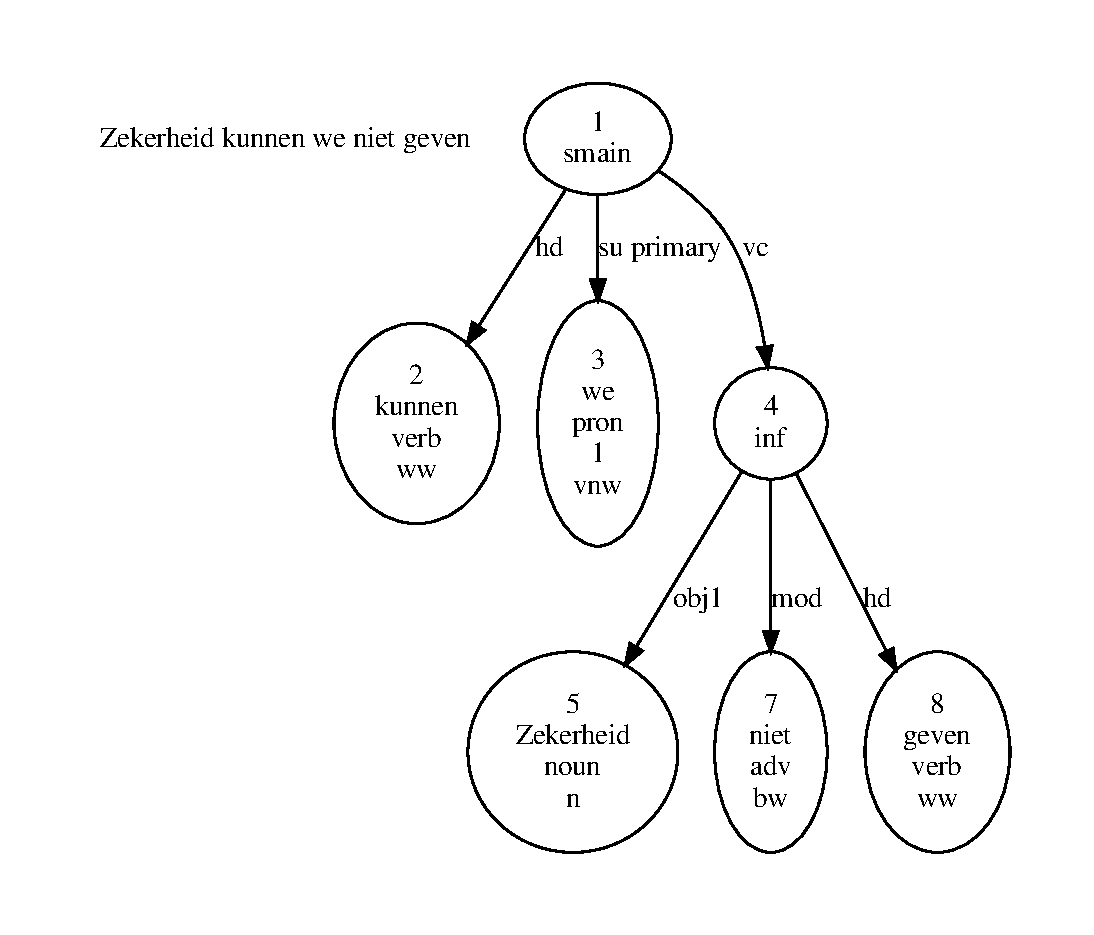
\includegraphics[scale=0.5]{zekerheid.pdf}
\end{figure}
\end{frame}
}

\begin{frame}{Extraction: Parameters}
\alert{Parameters}
\begin{itemize}
\item Translation Tables
	\begin{itemize}
		\item Atomic Types: POS \& Phrasal Category Tags \\
			\{\textit{np}: \textsc{np}, \textit{vnw}: \textsc{vnw}, \dots \}
		\item Implications: Dependency Labels \\
			\{\textit{su}: $\myrightarrow{su}$, \textit{obj}: $\myrightarrow{obj}$, \dots \}
	\end{itemize}
\item Head Dependencies \\
	\{\textit{hd}, \textit{rhd}, \textit{whd}, \textit{crd}, \textit{cmp}\}
\item Modifier Dependencies \\
	\{\textit{mod}, \textit{app}, \textit{predm}\}
\end{itemize}
\end{frame}

\begin{frame}{Extraction: Algorithm}
\alert{General Idea}
\begin{itemize}
\item[] For each branch
	\begin{itemize}
		\item Find phrasal head, dependants, modifiers
		\item Collect \& arrange dependant types
		\item Type head as a functor from argument types to parent type
		\item Type modifiers as morphisms from parent type to itself
	\end{itemize}
\end{itemize}
\end{frame}

{
\setbeamercolor{background canvas}{bg=gray!00}
\begin{frame}{Extraction: Example (1)}
\begin{figure}
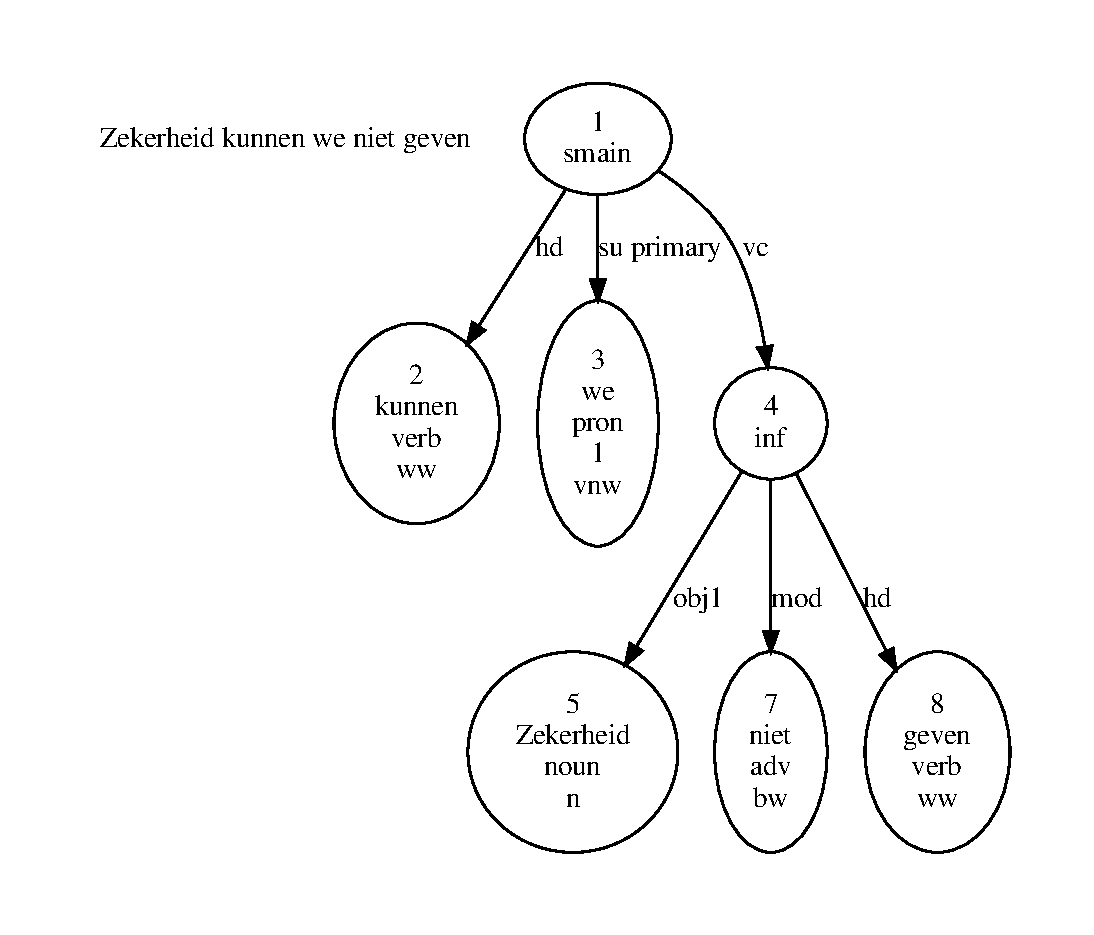
\includegraphics[scale=0.5]{zekerheid.pdf}
\end{figure}
\end{frame}
}

{
\setbeamercolor{background canvas}{bg=gray!00}
\begin{frame}{Extraction: Example (1)}
\begin{figure}
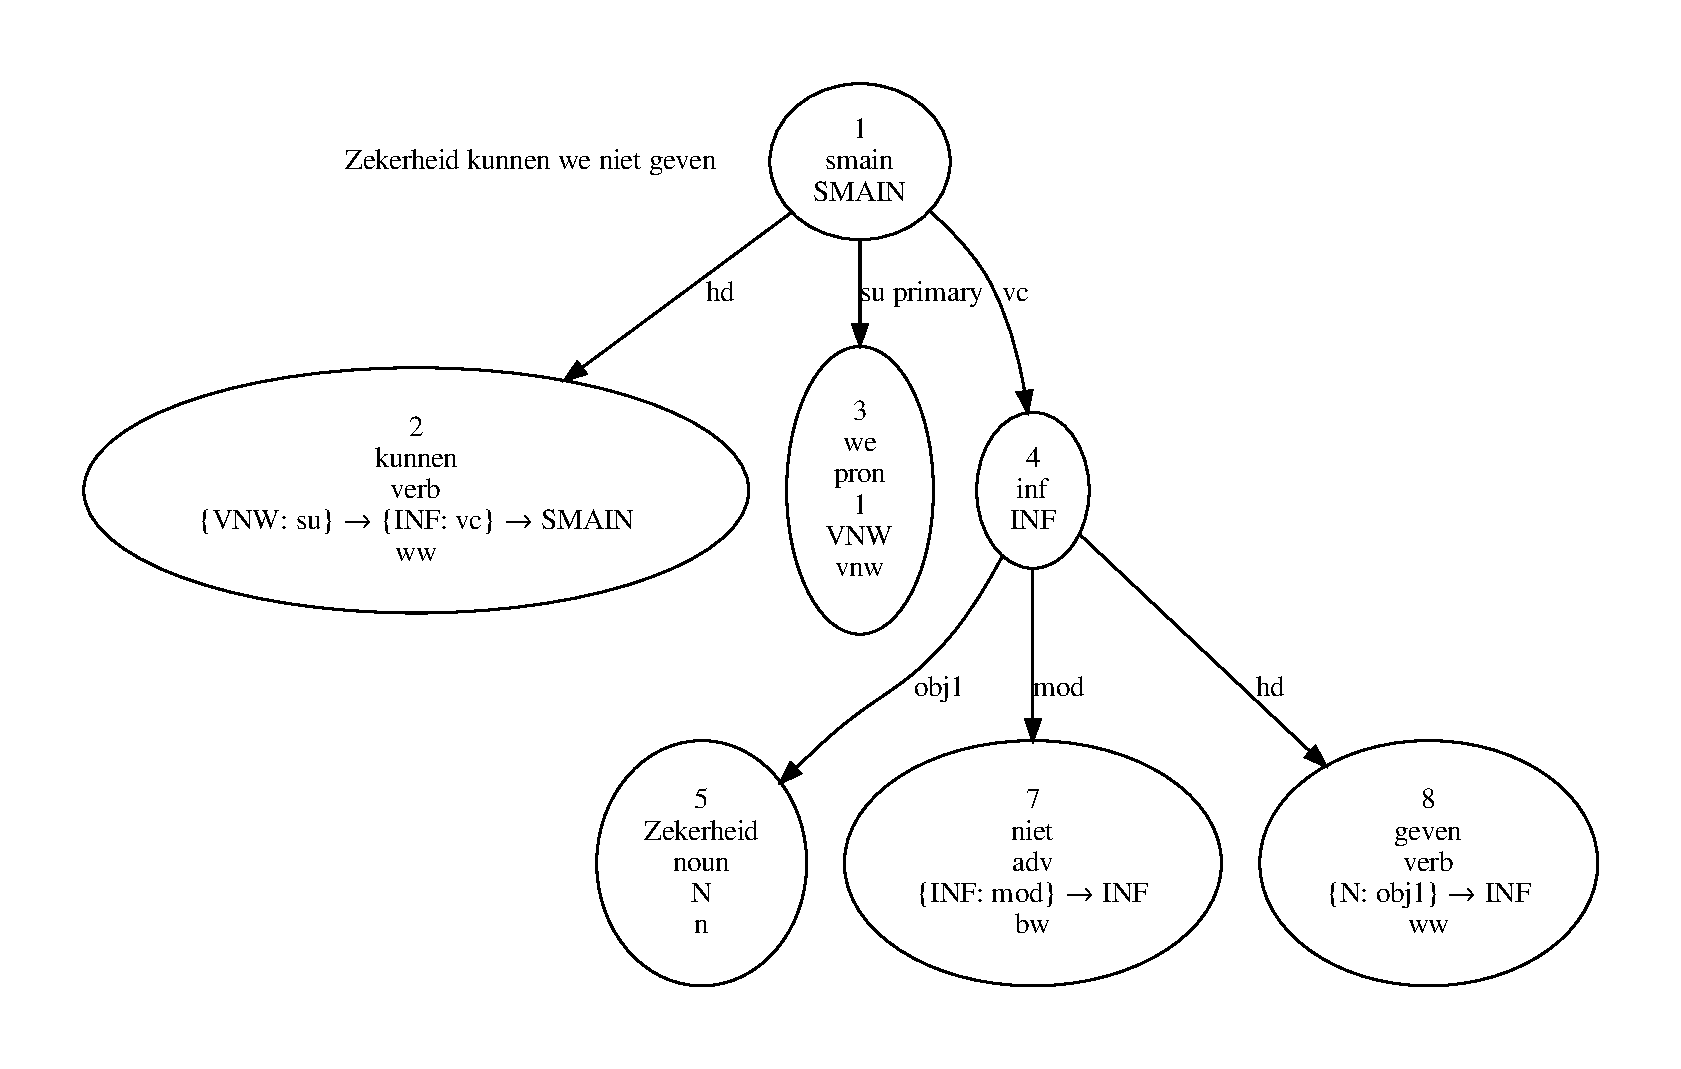
\includegraphics[scale=0.38]{zekerheid2.pdf}
\end{figure}
\end{frame}
}

{
\setbeamercolor{background canvas}{bg=gray!00}
\begin{frame}{Extraction: Example (2)}
\alert{Hypothetical Reasoning}
\begin{itemize}
\item[] \color{black}{When type assigning arguments, consider internal ``gaps''}
\end{itemize}

\begin{figure}
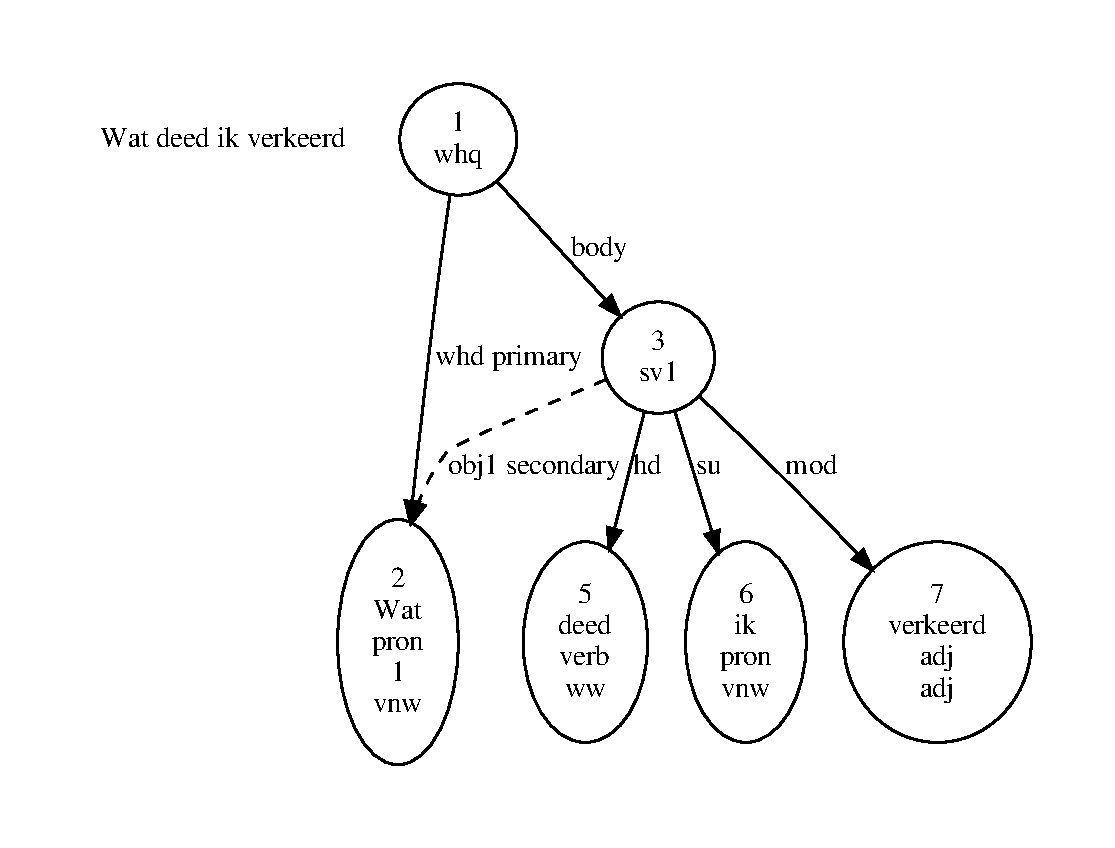
\includegraphics[scale=0.5]{deed.pdf}
\end{figure}
\end{frame}
}

{
\setbeamercolor{background canvas}{bg=gray!00}
\begin{frame}{Extraction: Example (2)}
\alert{Hypothetical Reasoning}
\begin{itemize}
\item[] \color{black}{When type assigning arguments, consider internal ``gaps''}
\end{itemize}

\begin{figure}
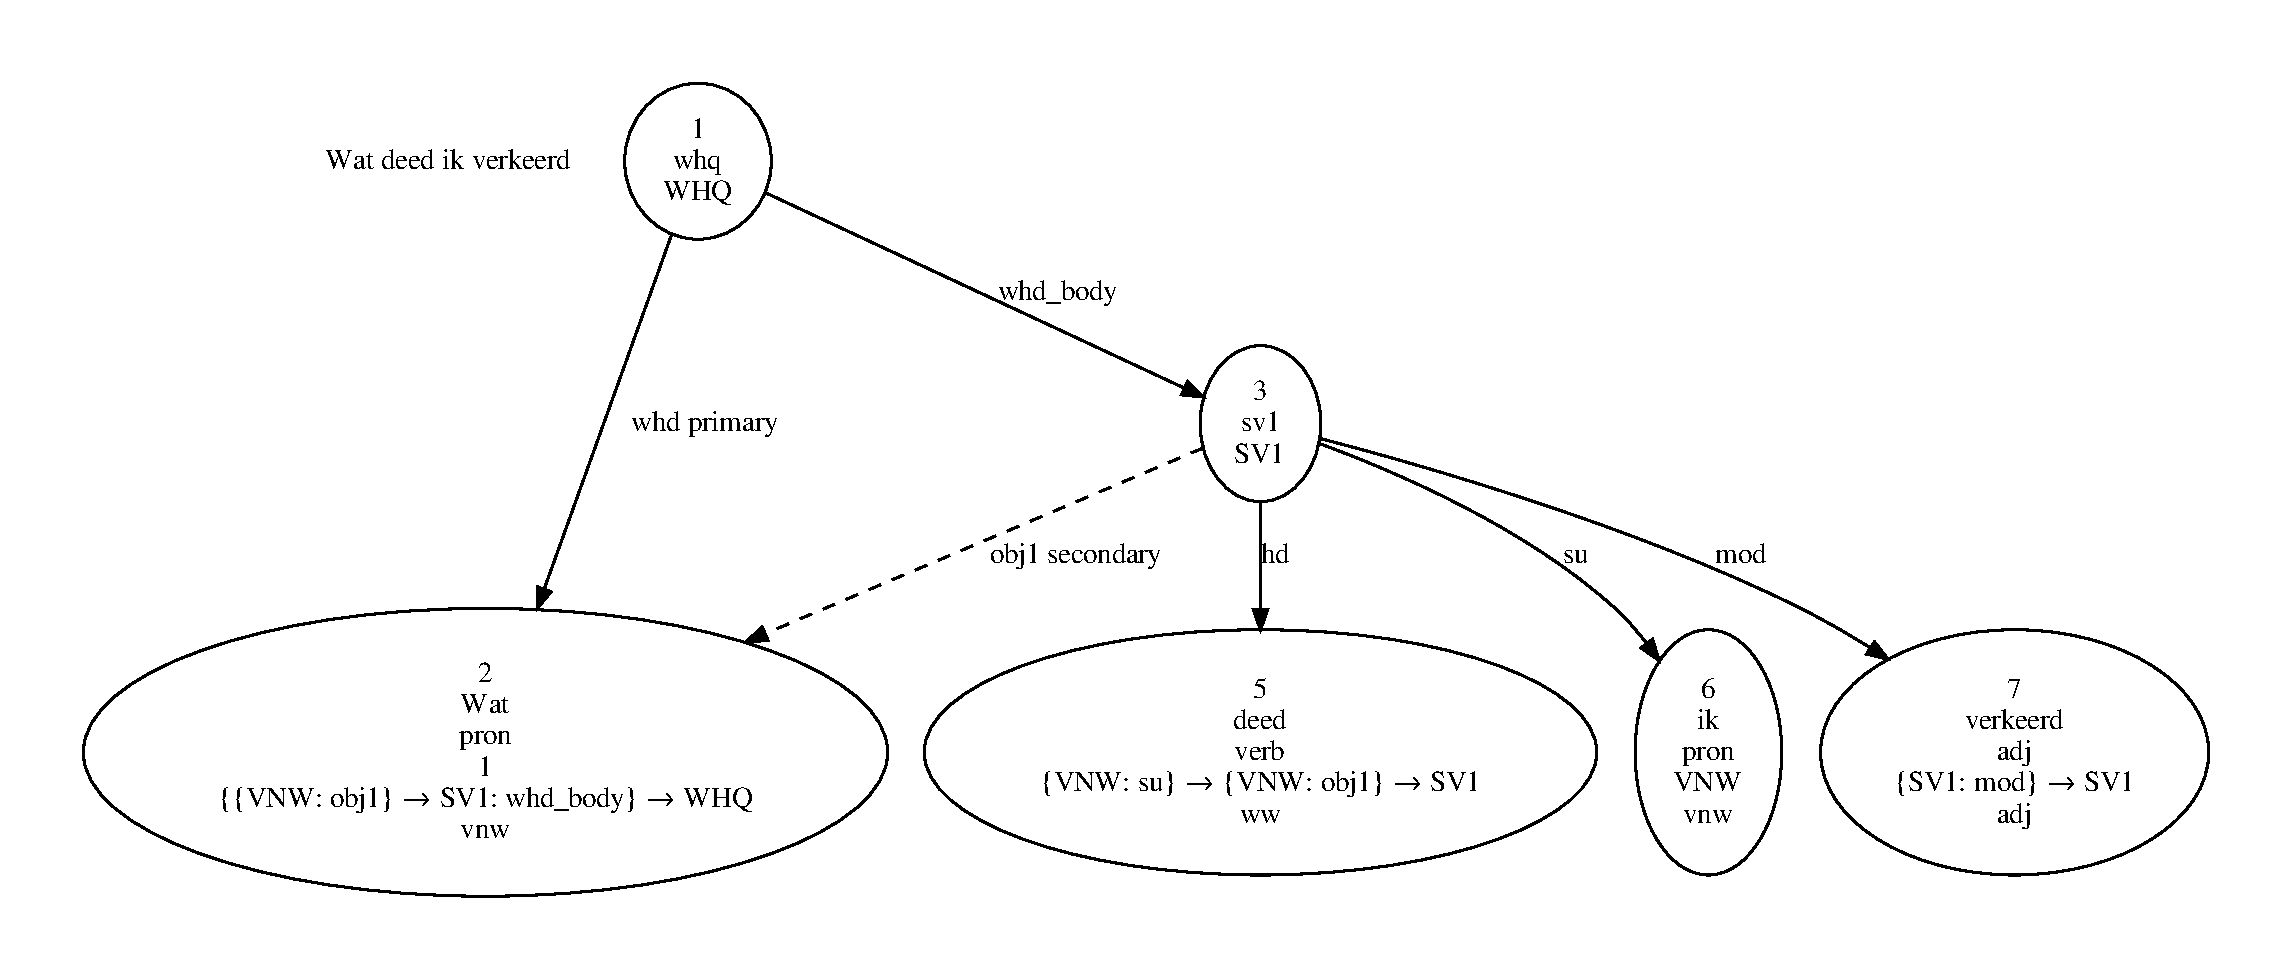
\includegraphics[scale=0.3]{deed2.pdf}
\end{figure}
\end{frame}
}

{
\setbeamercolor{background canvas}{bg=gray!00}
\begin{frame}{Extraction: Results (1)}
\centering
\vfill
\textcolor{black}{$\sim$ 5\,700 unique types}
\begin{figure}
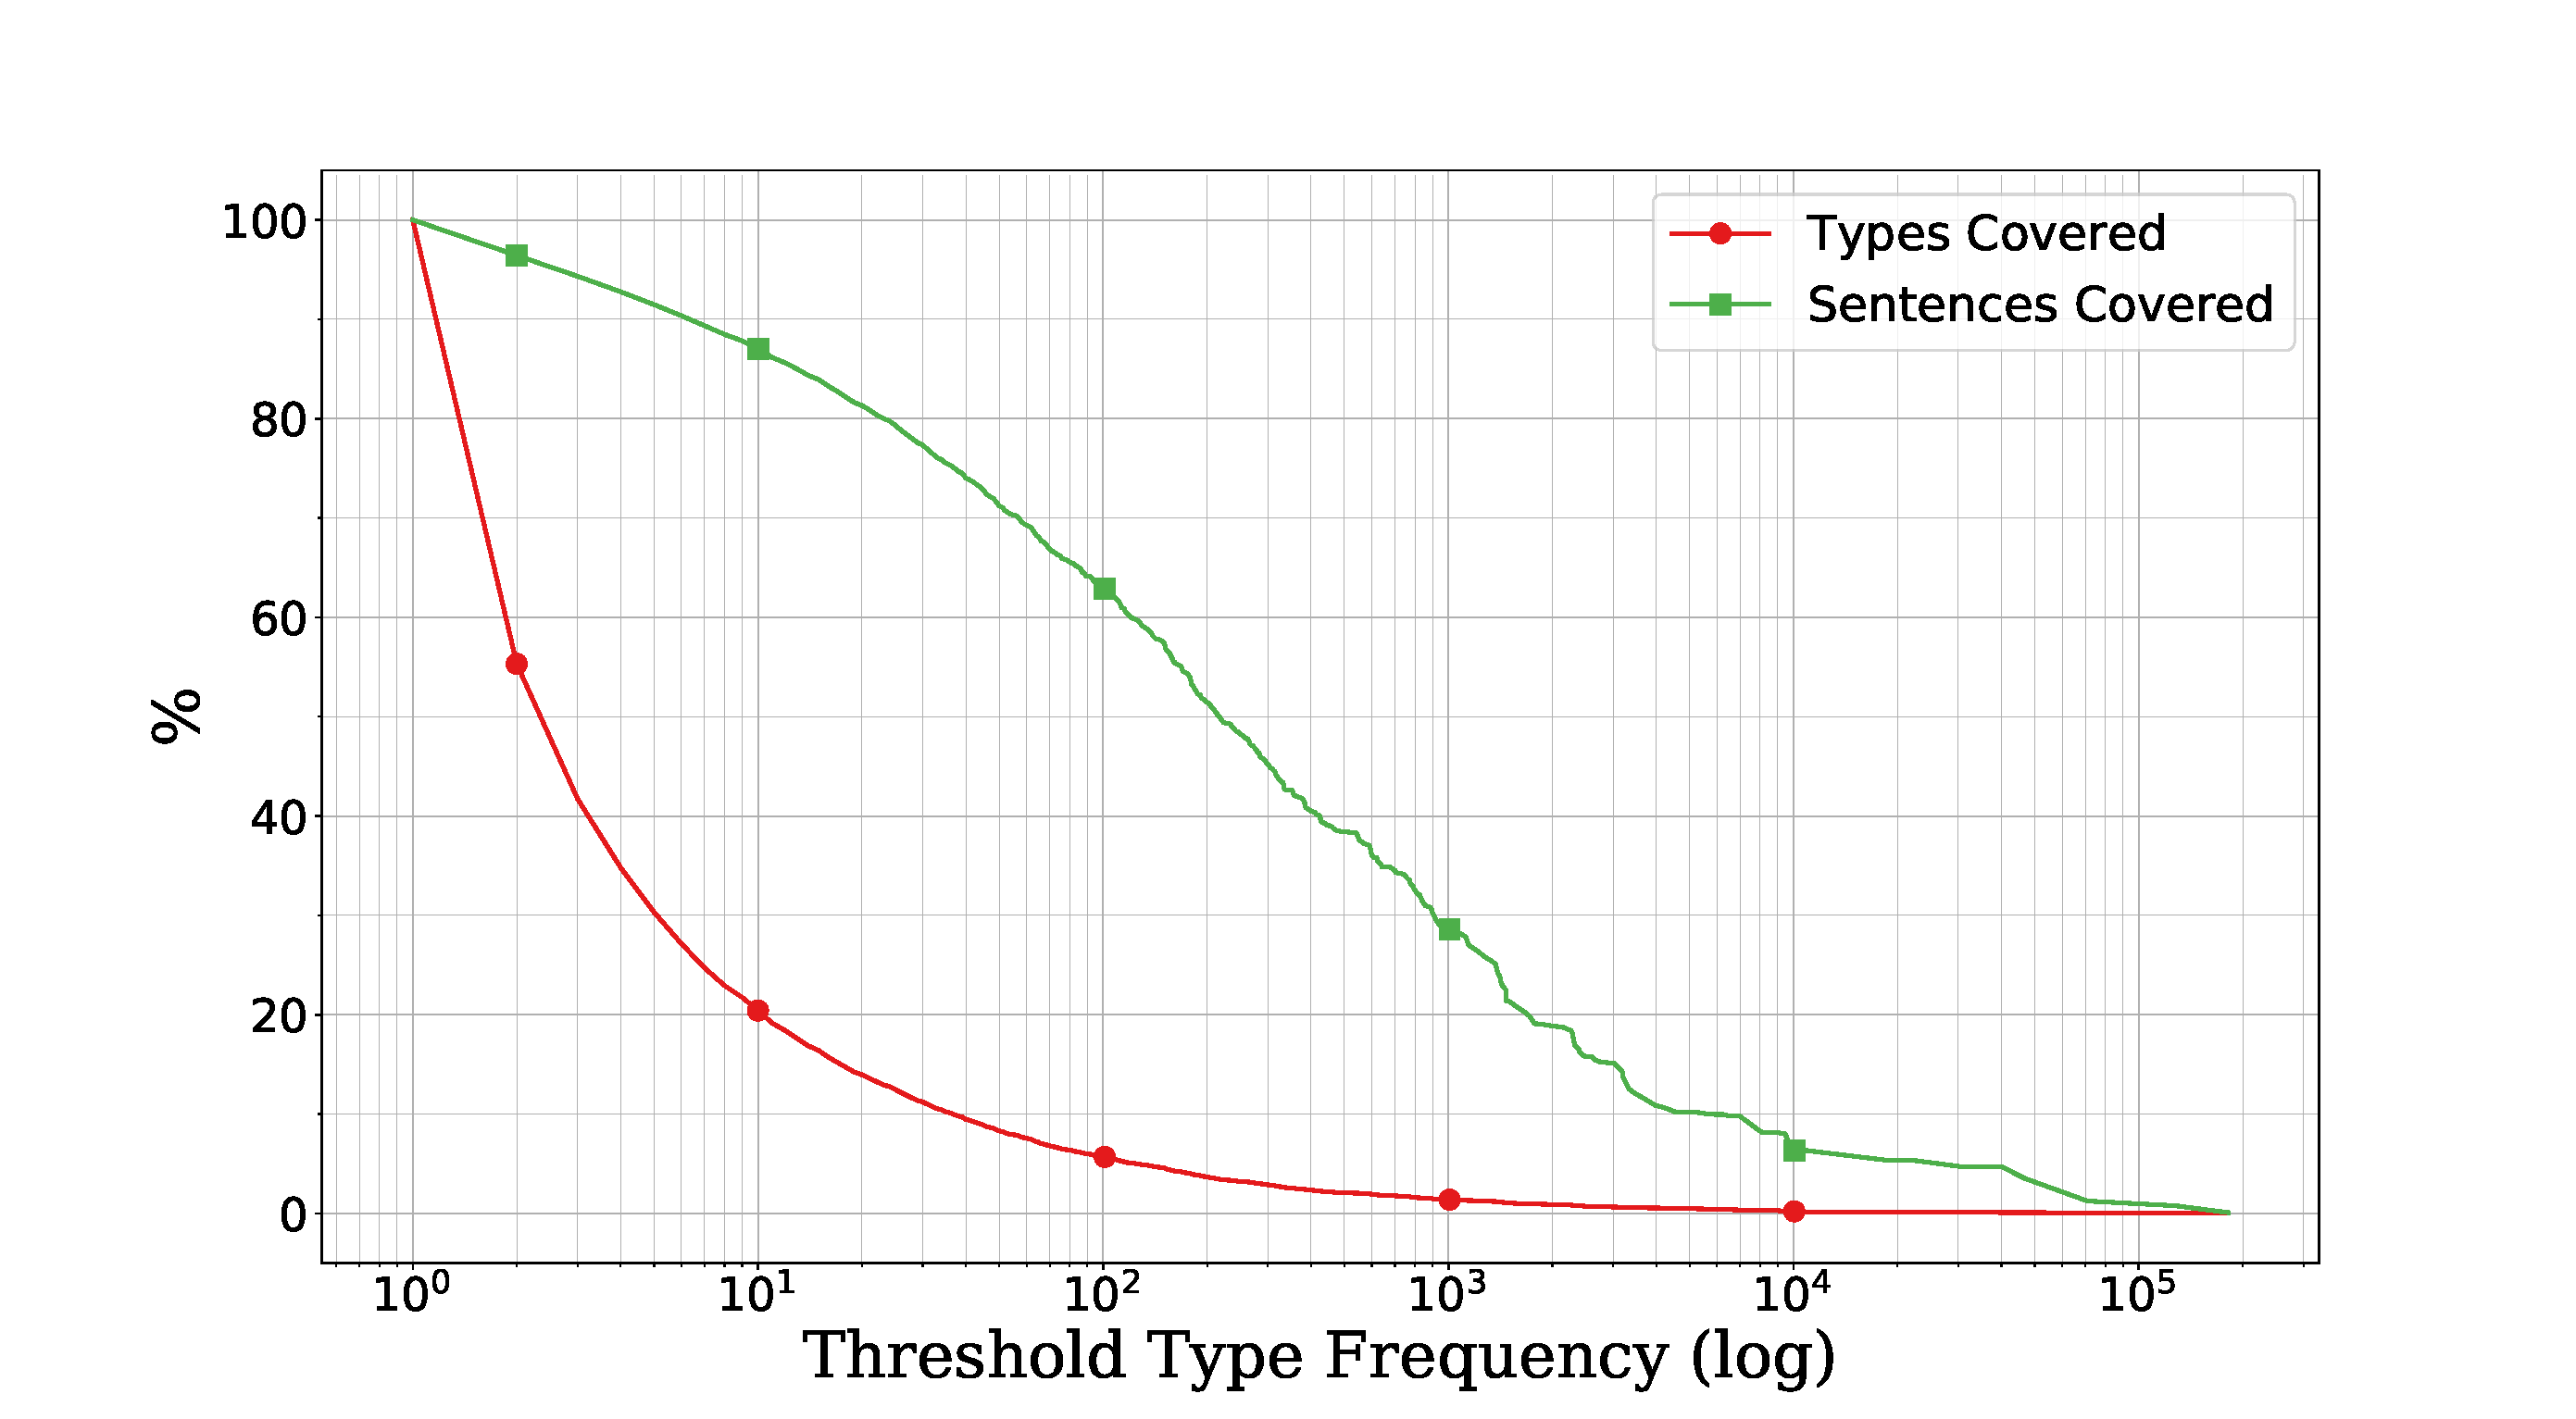
\includegraphics[scale=0.24]{sparsity.pdf}
\end{figure}
\end{frame}
}

{
\setbeamercolor{background canvas}{bg=gray!00}
\begin{frame}{Extraction: Results (2)}
\begin{figure}
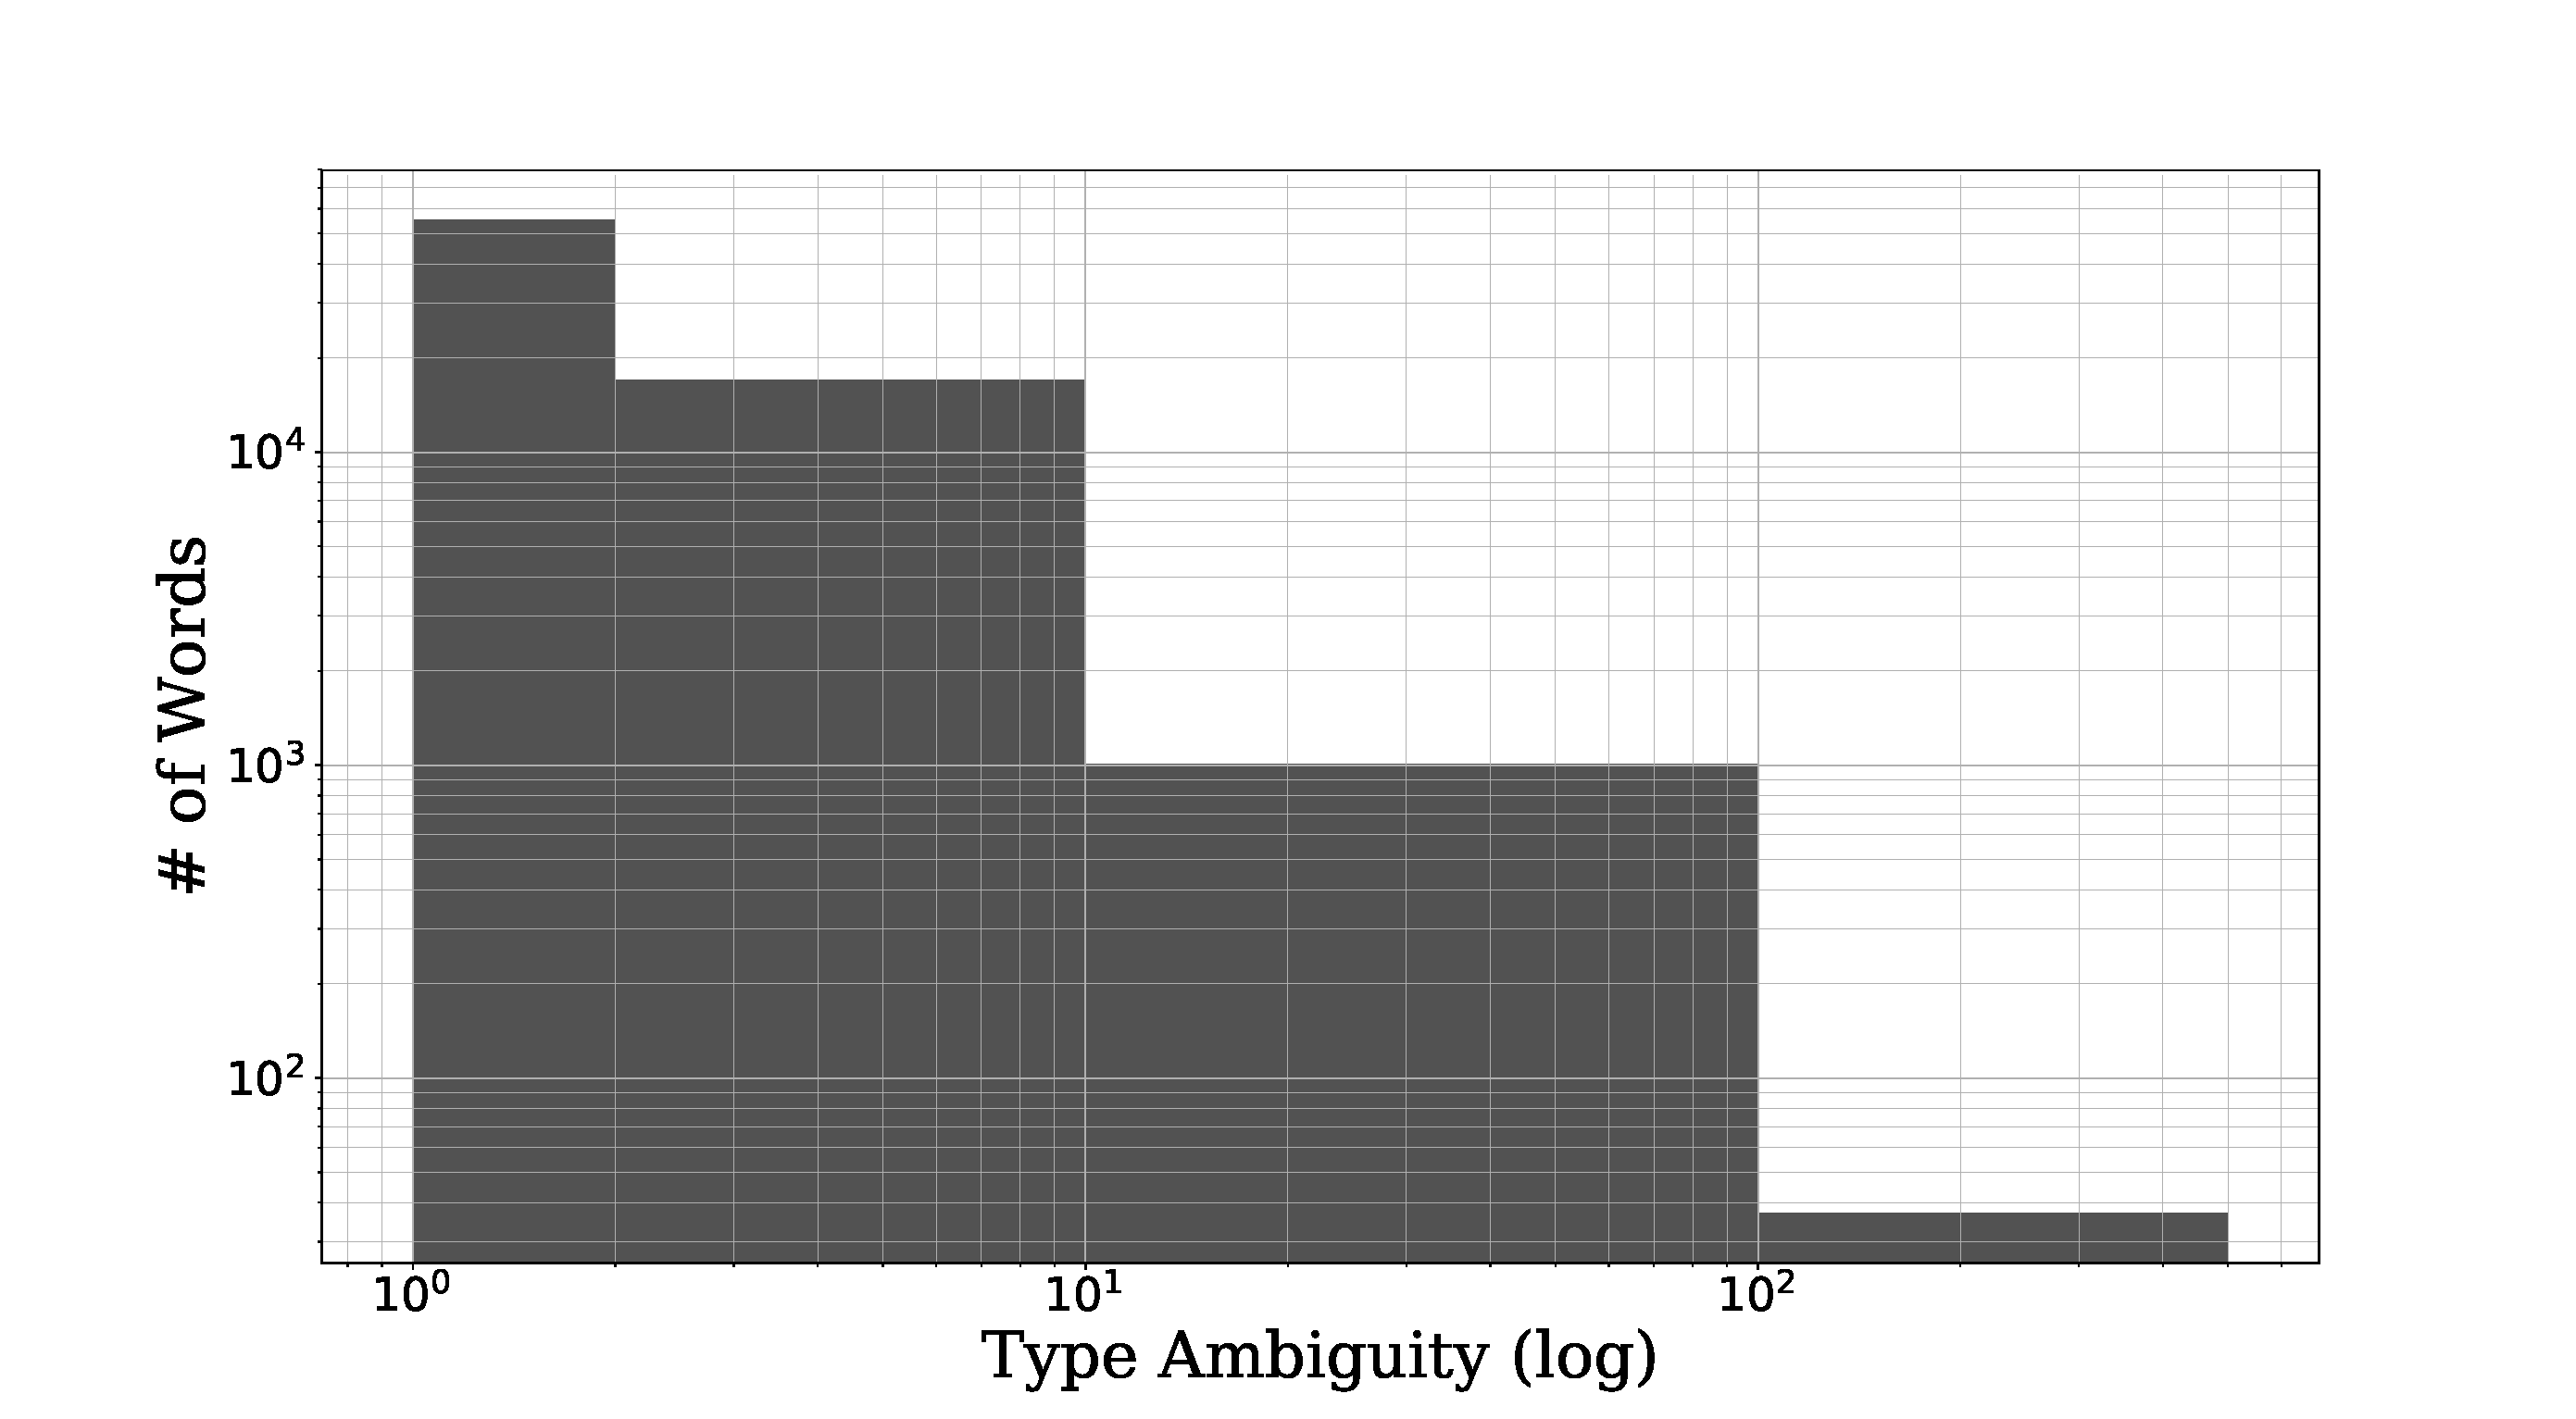
\includegraphics[scale=0.24]{ambiguity.pdf}
\end{figure}
\end{frame}
}

\section{Supertagging}

\begin{frame}{Supertagging: Standard Approach}
\alert{Sequence Classification}\\
\quad Given input data sequence (word vectors) \\
\quad predict a class for each sequence item (types)
\vfill

\pause
\begin{figure}
\centering
\begin{tikzpicture}
	
	\node[rectangle, inner sep=0pt, minimum width=120pt, minimum height=20pt] (ducks) at (-2, -1.5) {eenden};
	\node[rectangle, inner sep=0pt, minimum width=120pt, minimum height=20pt] (eat) at (0, -1.5) {eten};
	\node[rectangle, inner sep=0pt, minimum width=120pt, minimum height=20pt] (fish) at (2, -1.5) {vis};
	
	\node[draw=white, rectangle, minimum width=160pt, minimum height=20pt, ultra thick, fill=black] (bb) at (0, 0) {Black Rectangle};
	
	\pause
	\node[rectangle, inner sep=0pt, minimum width=120pt, minimum height=20pt] (ducks) at (-2, -1.5) {eenden};
	\node[rectangle, inner sep=0pt, minimum width=120pt, minimum height=20pt] (eat) at (0, -1.5) {eten};
	\node[rectangle, inner sep=0pt, minimum width=120pt, minimum height=20pt] (fish) at (2, -1.5) {vis};
	\draw ($(ducks.north) + (0, 0)$) edge[->, ultra thick] node[above] {} ($(bb.south) + (-2, 0)$);
	\draw ($(eat.north) + (0, 0)$) edge[->, ultra thick] node[above] {} ($(bb.south) + (0, 0)$);
	\draw ($(fish.north) + (0, 0)$) edge[->, ultra thick] node[above] {} ($(bb.south) + (2, 0)$);
	
	\pause
	\node[rectangle, inner sep=0pt, minimum width=120pt, minimum height=20pt] (ducktype) at (-2, 1.5) {\textsc{np}};
	\draw ($(ducktype.south) + (0, 0)$) edge[<-, ultra thick] node[above] {} ($(bb.north) + (-2, 0)$);
	\pause
	\node[rectangle, inner sep=0pt, minimum width=120pt, minimum height=20pt] (eattype) at (0, 1.5) {$\textsc{np} \myrightarrow{su} \textsc{np} \myrightarrow{obj} \textsc{s}$};
	\draw ($(eattype.south) + (0, 0)$) edge[<-, ultra thick] node[above] {} ($(bb.north) + (0, 0)$);
	\pause
	\node[rectangle, inner sep=0pt, minimum width=120pt, minimum height=20pt] (fishtype) at (2, 1.5) {$\textsc{np}$};
	\draw ($(fishtype.south) + (0, 0)$) edge[<-, ultra thick] node[above] {} ($(bb.north) + (2, 0)$);
\end{tikzpicture}
\end{figure}
\end{frame}

\begin{frame}{Supertagging: Standard Approach}
\alert{The Problem}
\begin{itemize}
	\item[] Can't predict unseen types
	\item[] Bad at predicting rare types
\end{itemize}
\end{frame}

\begin{frame}{Supertagging: An Alternative}
\alert{Type Syntax}\\
A CFG of two meta-rules
\begin{align*}
\{ (S & \implies A) \  \forall \ A \in \mathcal{A} \}\\
\{(S & \implies S \ \myrightarrow{d} \ S) \ \forall \ d \in \mathcal{D} \}
\end{align*}

\pause
CFGs: learnable \\ 
Supertagging: learnable \\
\pause
CFG embedded within supertagging: learnable..?\\
\quad ..if so, \alert{unbounded co-domain} supertagging
\end{frame}

\begin{frame}{Supertagging: Unbounded co-domain}

\alert{Reformulation}\\
\quad Given input data sequence (word vectors) \\
\quad generate an output sequence (atomic types \& binary connectives)
\vfill

\pause
\begin{figure}
\centering
\begin{tikzpicture}
	
	\node[rectangle, inner sep=0pt, minimum width=120pt, minimum height=20pt] (ducks) at (-2, -1.5) {eenden};
	\node[rectangle, inner sep=0pt, minimum width=120pt, minimum height=20pt] (eat) at (0, -1.5) {eten};
	\node[rectangle, inner sep=0pt, minimum width=120pt, minimum height=20pt] (fish) at (2, -1.5) {vis};
	
	\node[draw=white, rectangle, minimum width=160pt, minimum height=20pt, ultra thick, fill=black] (bb) at (0, 0) {Better Black Rectangle};
	
	\pause
	\node[rectangle, inner sep=0pt, minimum width=120pt, minimum height=20pt] (ducks) at (-2, -1.5) {eenden};
	\node[rectangle, inner sep=0pt, minimum width=120pt, minimum height=20pt] (eat) at (0, -1.5) {eten};
	\node[rectangle, inner sep=0pt, minimum width=120pt, minimum height=20pt] (fish) at (2, -1.5) {vis};
	\draw ($(ducks.north) + (0, 0)$) edge[->, ultra thick] node[above] {} ($(bb.south) + (-2, 0)$);
	\draw ($(eat.north) + (0, 0)$) edge[->, ultra thick] node[above] {} ($(bb.south) + (0, 0)$);
	\draw ($(fish.north) + (0, 0)$) edge[->, ultra thick] node[above] {} ($(bb.south) + (2, 0)$);
	
	\pause
	\node[rectangle, inner sep=0pt, minimum width=120pt, minimum height=20pt] (npone) at (-2.5, 1.5) {\textsc{np}};
	\draw ($(npone.south) + (0, 0)$) edge[<-, ultra thick] node[above] {} ($(bb.north) + (-2.5, 0)$);
	\pause
	\node[rectangle, inner sep=0pt, minimum width=120pt, minimum height=20pt] (spone) at (-2, 1.5) {\#};
	\draw ($(spone.south) + (0, 0)$) edge[<-, ultra thick] node[above] {} ($(bb.north) + (-2, 0)$);
	\pause
	\node[rectangle, inner sep=0pt, minimum width=120pt, minimum height=20pt] (nptwo) at (-1.5, 1.5) {\textsc{np}};
	\draw ($(nptwo.south) + (0, 0)$) edge[<-, ultra thick] node[above] {} ($(bb.north) + (-1.5, 0)$);
	\pause
	\node[rectangle, inner sep=0pt, minimum width=120pt, minimum height=20pt] (su) at (-1, 1.5) {$\myrightarrow{su}$};
	\draw ($(su.south) + (0, 0)$) edge[<-, ultra thick] node[above] {} ($(bb.north) + (-1, 0)$);
	\pause
	\node[rectangle, inner sep=0pt, minimum width=120pt, minimum height=20pt] (npthree) at (-0.5, 1.5) {$\textsc{np}$};
	\draw ($(npthree.south) + (0, 0)$) edge[<-, ultra thick] node[above] {} ($(bb.north) + (-0.5, 0)$);
	\pause
	\node[rectangle, inner sep=0pt, minimum width=120pt, minimum height=20pt] (obj) at (-0, 1.5) {$\myrightarrow{obj}$};
	\draw ($(obj.south) + (0, 0)$) edge[<-, ultra thick] node[above] {} ($(bb.north) + (-0, 0)$);	
	\pause
	\node[rectangle, inner sep=0pt, minimum width=120pt, minimum height=20pt] (s) at (0.5, 1.5) {$\textsc{s}$};
	\draw ($(s.south) + (0, 0)$) edge[<-, ultra thick] node[above] {} ($(bb.north) + (0.5, 0)$);
	\pause
	\node[rectangle, inner sep=0pt, minimum width=120pt, minimum height=20pt] (spltwo) at (1, 1.5) {\#};
	\draw ($(spltwo.south) + (0, 0)$) edge[<-, ultra thick] node[above] {} ($(bb.north) + (1, 0)$);	
	\pause
	\node[rectangle, inner sep=0pt, minimum width=120pt, minimum height=20pt] (npend) at (1.5, 1.5) {$\textsc{np}$};
	\draw ($(npend.south) + (0, 0)$) edge[<-, ultra thick] node[above] {} ($(bb.north) + (1.5, 0)$);	
		
	
\end{tikzpicture}
\end{figure}
\end{frame}

\begin{frame}{Supertagging: Unbounded co-domain}
\alert{Requirements}
\begin{itemize}
\item Global Receptive Field (long-distance dependencies)
\item Auto-Regressive (output conditional on prior output)	
\end{itemize}

\pause
\alert{Options}
\begin{itemize}
\item RNN encoder-decoder \pause {\color{red}Fixed-length compression}
\item RNN encoder-separable decoder \pause {\color{red}Only locally auto-regressive}
\item Self-Attentive encoder-decoder \pause {\color{green}\checkmark}
\end{itemize}
\end{frame}

\begin{frame}[standout]{Supertagging: Model}
\begin{figure}
\centering
	\scalebox{0.8}{
		\begin{tikzpicture}[every text node part/.style={align=center},
		 every node/.style={transform shape},
		 scale=0.6,
		block/.style={rectangle, inner sep=0pt, minimum width=120pt, minimum height=60pt, rounded corners, ultra thick},
		str/.style={rectangle, inner sep=0pt, minimum width=120pt, minimum height=20pt},
		arrow/.style={->, ultra thick},
		pwise/.style={circle, inner sep=0pt, minimum size=10pt},
		smallblock/.style={circle, inner sep=5pt, minimum size=12pt, rounded corners, thick}]
		
			\node[str] (sentence) at (0, 5) {Input Sentence};		
			\node[str] (symbols) at (7.5, 5) {Output Sequence};
		
		    \definecolor{first}{RGB}{82,82,82}
		    \definecolor{enc}{RGB}{253,192,134}
		    \definecolor{dec}{RGB}{127,201,127}
		    \definecolor{dec2}{RGB}{140,220,140}
		    \definecolor{emb}{RGB}{190,174,212}
		
			\node[block, draw=black, fill=gray!10, draw=gray!130] (elmo) at (0,8) {\textcolor{gray!110}{ELMo}};
			\node[block, draw=black, fill=enc] (te) at (0,12) {\textbf{Encoder}};
			\node[block, draw=black, fill=emb] (se) at (7.5,8) {\textbf{Embedding}};
			\node[block, draw=black, fill=dec2] (td2) at (7.75, 12.25) {};
			\node[block, draw=black, fill=dec] (td) at (7.5,12) {\textbf{Decoder}};
			\node[block, draw=black, fill=emb] (set) at (15,12) {\textbf{Embedding}\\ (transposed)};	
			\node[smallblock, draw=black] (ss) at (15, 8) {$\sigma$};
			\node[smallblock, draw=black] (am) at (12, 8) {$\alpha$};
			\node[str] (out) at (15,5) {Output Probabilities};	
			
		
			\draw (symbols) edge [arrow, gray!130] node[right] {M symbols} (se);
			\draw  (sentence) edge [arrow, gray!130] node[left] {N words} (elmo);
			\draw  (elmo) edge [arrow, gray!130] node[left] {\small Sentence Embedding\\ $\mathbb{R} ^ {N \times 1024}$} (te);
			\draw  (se) edge [arrow] node[right] {\small Symbol Embeddings\\ $\mathbb{R} ^ {M \times 1024}$} (td);
			\draw ($(te.east) + (0, 0.5)$) edge [arrow] node[above] {\small Encoder Keys\\ $\mathbb{R}^ {N \times 1024}$} ($(td.west) + (0, 0.5)$);
			\draw ($(te.east) + (0, -0.5)$) edge [arrow] node[below] {\small Encoder Values\\ $\mathbb{R}^ {N \times 1024}$} ($(td.west) + (0, -0.5)$);\
			\draw ($(td.east) + (0.25, 0)$) edge [arrow] node[above] {\small Decoder Values\\ $\mathbb{R}^ {M \times 1024}$} (set);
			\draw (set) edge [arrow] node[right] {\small Class Weights} (ss);
			\draw (ss) edge [arrow] (out);
			\draw (set.south) [dotted, very thick] .. controls +(-1,0) and +(-0.5, 0.5) .. (am.north);
			\draw (am.south) [dotted, very thick, ->] .. controls +(0,-0.5) and +(2, ) .. (symbols.east);
		\end{tikzpicture}
	}
\end{figure}
\end{frame}

{
\setbeamercolor{background canvas}{bg=gray!00}
\begin{frame}{Supertagging: Evaluation}

\small
\hspace{20pt}
\color{black}{
\begin{tabularx}{0.7\textwidth}{@{}csssss@{}}
	{} & \multicolumn{5}{c}{\centering Frequency}\\
	{} & \small Overall & \small Unseen & \small  Rare & \small Mid & \small High \\
	\cmidrule[0.001em]{2-6}
	Accuracy & \textbf{ 88.05} & \color{red}{\textbf{19.2}} & \textbf{45.68} & \textbf{65.62} & \textbf{89.93}\\
\end{tabularx}\hfill
}

	\begin{figure}	
	\hspace{-35pt}
	\vspace{30pt}
	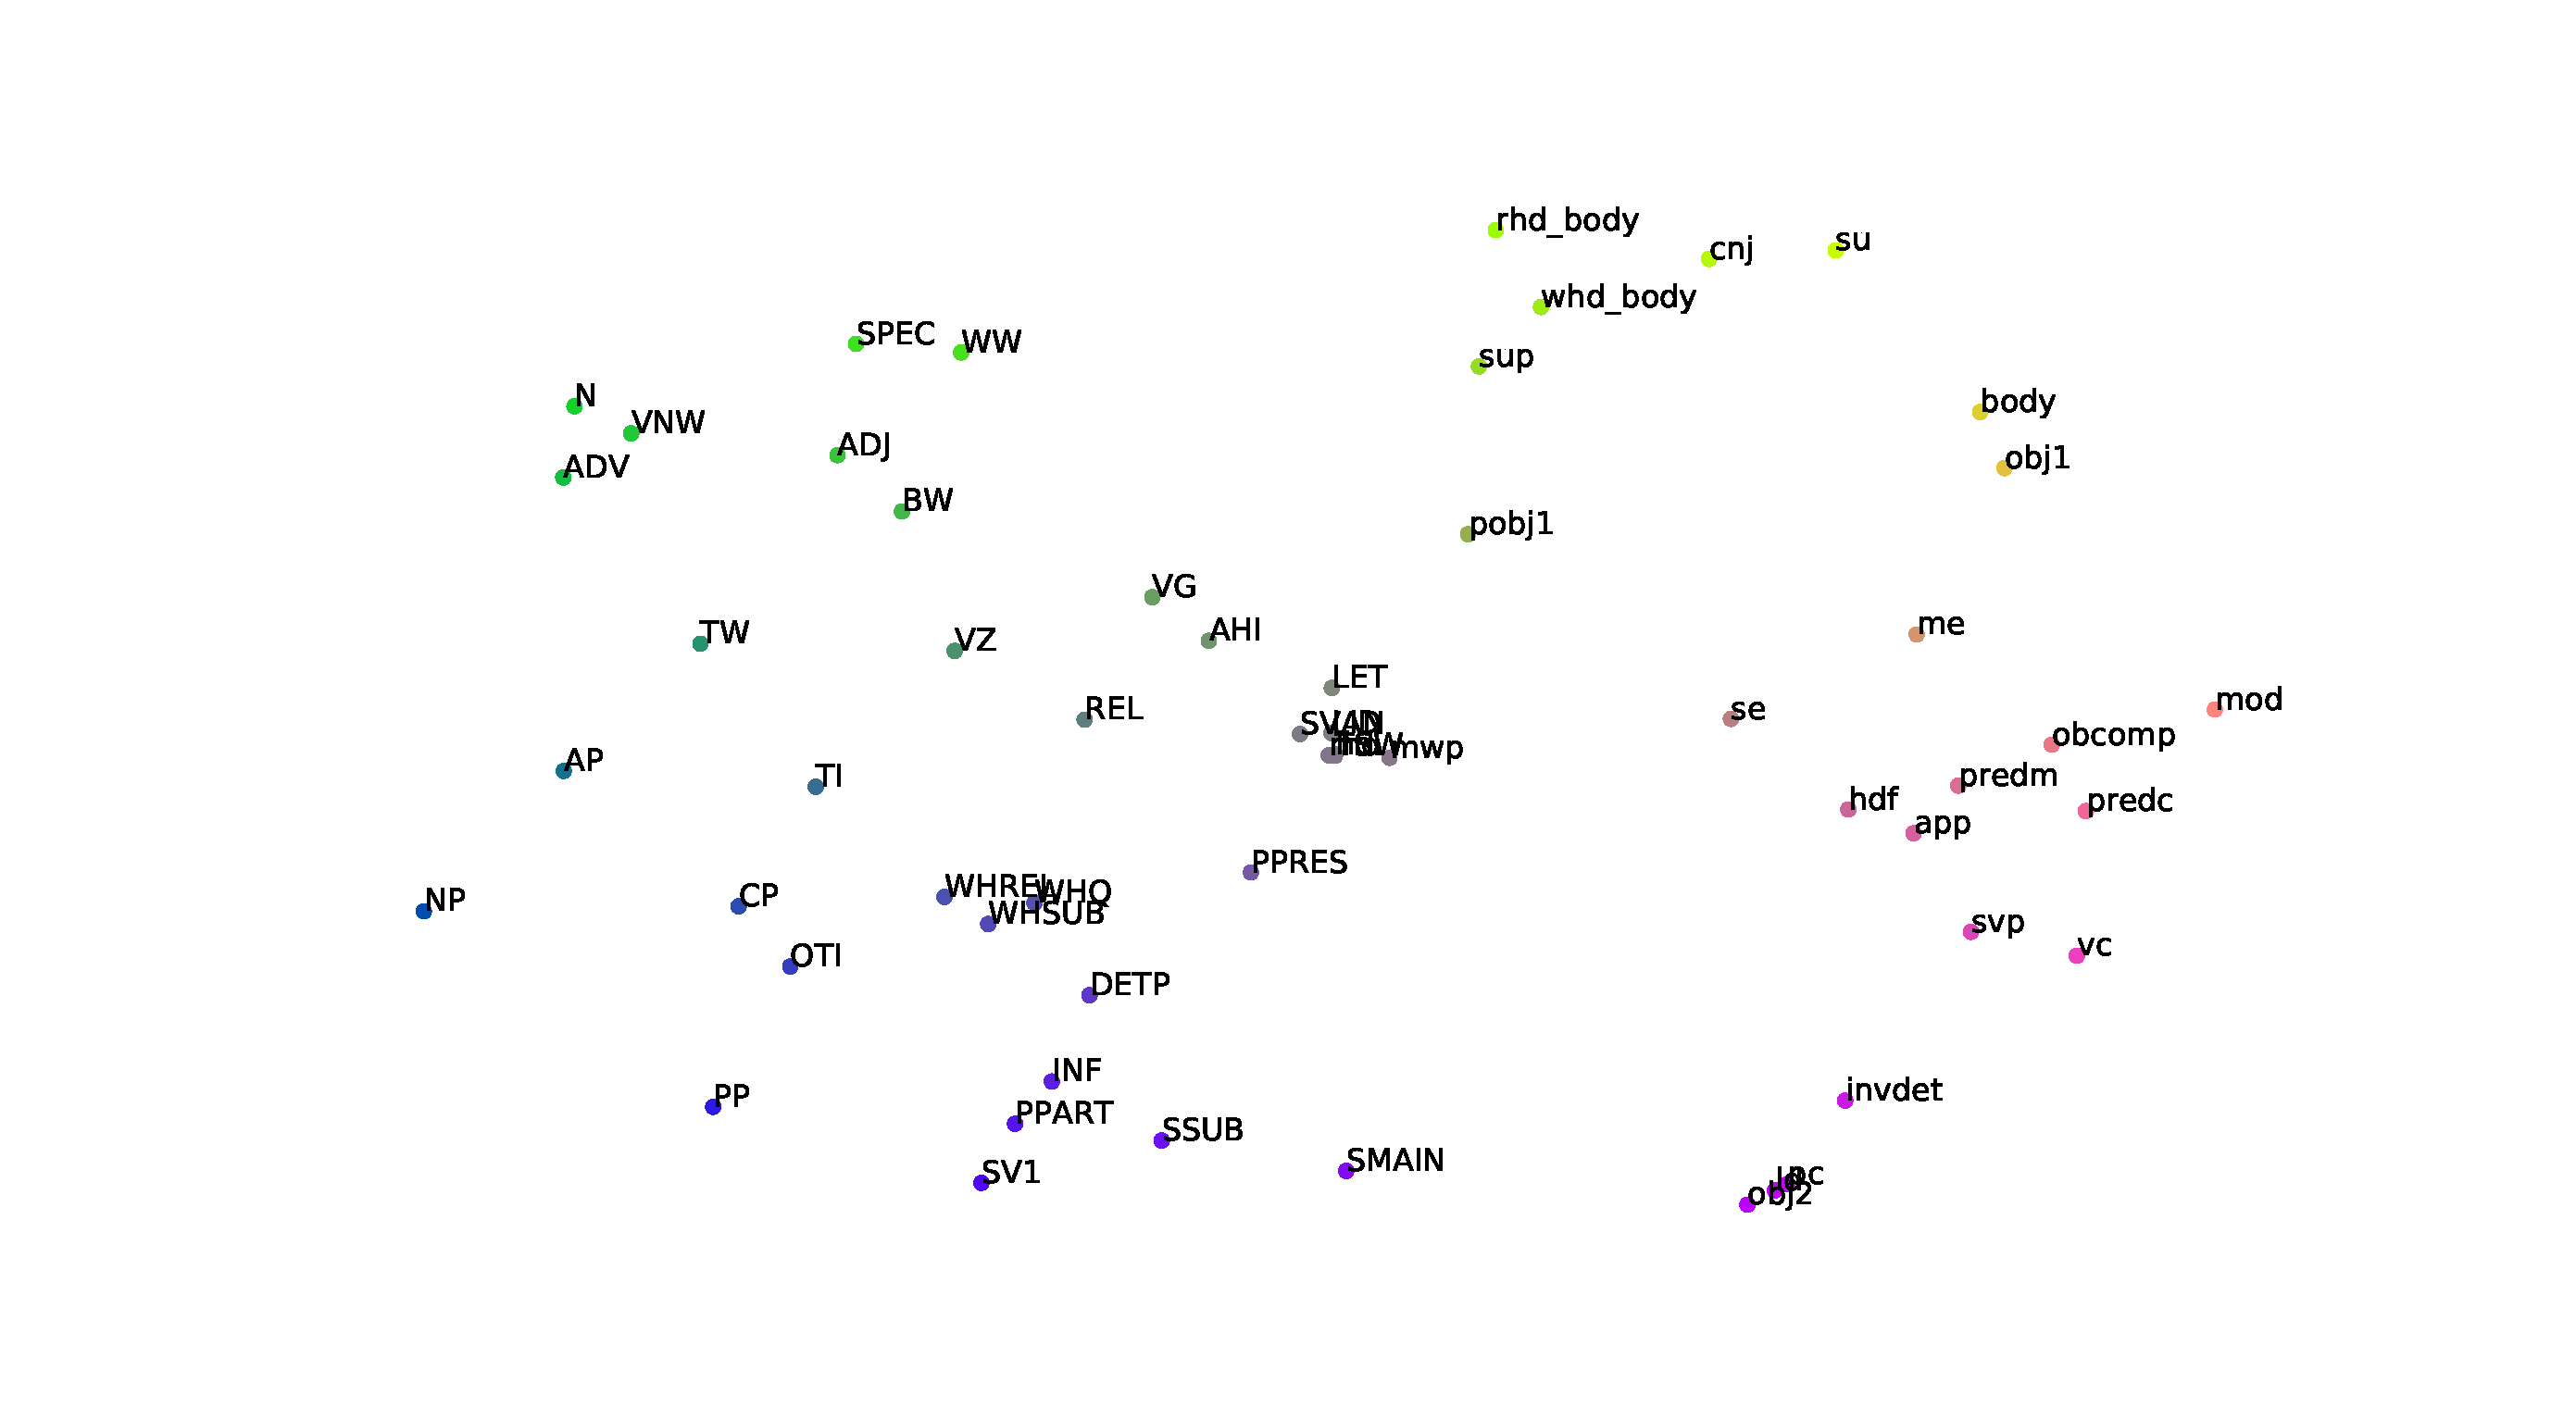
\includegraphics[scale=0.25]{cluster.pdf}
\end{figure}	

\end{frame}
}

\section{Parsing}

\begin{frame}{Parsing: Intro}
\alert{Goal}\\
From abstract syntax to surface syntax	

\pause
\alert{Parse $\equiv$ Proof} \\
How can we efficiently navigate the proof space?
\end{frame}

\begin{frame}{Parsing: General Framework}
\alert{Parse State}
\begin{itemize}
	\item[] A logical judgement
	\item[] Word associations for (some) premises
	\item[] A lookahead containing last rule applied
\end{itemize}

\alert{Algorithm}\\
Given a parse state
\begin{itemize}
\item[1] Decide between introduction and elimination
\item[2] Perform either
\item[3] Update state(s)
\item[4] Repeat
\end{itemize}
\end{frame}

\begin{frame}{Parsing: Elimination}
Given a sequence of word \& type pairs \\ 
\quad Split into two disjoint sequences.. \\
\pause
\quad ..by assigning each item one of two labels
\end{frame}

\begin{frame}[standout]{Parsing: Model \& Results}
\begin{figure}
\scalebox{0.7}{
	\begin{tikzpicture}[every text node part/.style={align=center},
		 every node/.style={transform shape},
		 scale=0.7,
		block/.style={rectangle, inner sep=0pt, minimum width=120pt, minimum height=20pt, rounded corners, ultra thick},
		str/.style={rectangle, inner sep=0pt, minimum width=120pt, minimum height=20pt},
		arrow/.style={->, thick},
		pwise/.style={circle, inner sep=0pt, minimum size=10pt},
		smallblock/.style={circle, inner sep=5pt, minimum size=12pt, rounded corners, thick},
		mediumblock/.style={rectangle, inner sep=0pt, minimum width=30pt, minimum height=20pt, rounded corners, ultra thick},
		mini/.style={rectangle, inner sep=0pt, minimum width=30pt, minimum height=20pt, thick, draw=black,}]
		
		%	\node[str] (sentence) at (0, 5) {Input Sentence};
		%	\node[str] (symbols) at (7.5, 5) {Input Type Sequences};
		%	\node[str] (goal) at (13, 5) {Input Goal};
		\node[str] (sentence) at (4, -0.5) {Input Sentence};
		\node[str] (dog) at (3, 0) {};
		\node[str] (bites) at (4, 0) {};
		\node[str] (man) at (5, 0) {};
		
		\node[block, draw=gray!130, fill=gray!10] (elmo) at (4, 1.5) {\textcolor{gray!110}{ELMo}};
		
		\draw (dog) edge[arrow, gray!130] ($(elmo.south) + (-1, 0)$);
		\draw (bites) edge[arrow, gray!130] (elmo);
		\draw (man) edge[arrow, gray!130] ($(elmo.south) + (1, 0)$);
		
		\node[str] (w1) at (3, 3) {$\overrightarrow{w_1}$};
		\node[str] (w2) at (4, 3) {$\overrightarrow{w_2}$};
		\node[str] (w3) at (5, 3) {$\overrightarrow{w_3}$};
		
		\draw ($(elmo.north) + (-1, 0)$) edge[arrow, black] (w1);
		\draw (elmo) edge[arrow, black] (w2);
		\draw ($(elmo.north) + (1, 0)$) edge[arrow, black] (w3);
		
		\node[str] (types) at (11, -0.5) {Input Type Sequences};
		\node[str] (su) at (9, 0) {};
		\node[str] (verb) at (11, 0) {};
		\node[str] (obj) at (13, 0) {};
		
		\node[str] (t1) at (9, 3) {$\overrightarrow{t_1}$};
		\node[str] (t2) at (11, 3) {$\overrightarrow{t_2}$};
		\node[str] (t3) at (13, 3) {$\overrightarrow{t_3}$};
		
		\node[mediumblock, draw=black] (T1) at (9, 1.5) {$\pmb{\mathcal{T}}$};
		\node[mediumblock, draw=black] (T2) at (11, 1.5) {$\pmb{\mathcal{T}}$};
		\node[mediumblock, draw=black] (T3) at (13, 1.5) {$\pmb{\mathcal{T}}$};
		
		\draw (su) edge[arrow, gray!130] (T1);
		\draw (T1) edge[arrow, black] (t1);
		\draw (verb) edge[arrow, gray!130] (T2);
		\draw (T2) edge[arrow, black] (t2);
		\draw (obj) edge[arrow, gray!130] (T3);
		\draw (T3) edge[arrow, black] (t3);
		
		\node[str] (goal) at (17, -0.5) {Input Goal Type};
		\node[str] (g) at (17, 0) {};
		\node[str] (gt) at (17, 3) {$\overrightarrow{g}$};
		\node[mediumblock, draw=black] (T4) at (17, 1.5) {$\pmb{\mathcal{T}}$};
		\draw (g) edge[arrow, black] (T4);
		\draw (T4) edge[arrow, black] (gt);
		
		\node[str] (wtg1) at (9, 5) {$\overrightarrow{w_1};\overrightarrow{t_1};\overrightarrow{g}$};
		\node[str] (wtg2) at (11, 5) {$\overrightarrow{w_2};\overrightarrow{t_2};\overrightarrow{g}$};
		\node[str] (wtg3) at (13, 5) {$\overrightarrow{w_3};\overrightarrow{t_3};\overrightarrow{g}$};
		
		\draw (w1.north) edge[arrow, ultra thin, dashed] ($(wtg1.south) + (-0.7, 0)$);
		\draw (w2.north) edge[arrow, ultra thin, dashed] ($(wtg2.south) + (-0.7, 0)$);
		\draw (w3.north) edge[arrow, ultra thin, dashed] ($(wtg3.south) + (-0.7, 0)$);
		
		\draw (t1.north) edge[arrow, ultra thin, dashed] (wtg1.south);
		\draw (t2.north) edge[arrow, ultra thin, dashed] (wtg2.south);
		\draw (t3.north) edge[arrow, ultra thin, dashed] (wtg3.south);
		
		\draw (gt.north) edge[arrow, ultra thin, dashed] ($(wtg1.south) + (0.7, 0)$);
		\draw (gt.north) edge[arrow, ultra thin, dashed] ($(wtg2.south) + (0.7, 0)$);
		\draw (gt.north) edge[arrow, ultra thin, dashed] ($(wtg3.south) + (0.7, 0)$);
		
		\node[block, draw=black, minimum width=160pt] (RNN2) at (11.25, 7.25) {};
		\node[block, draw=black, minimum width=160pt, fill=white] (RNN) at (11, 7) {$\pmb{\mathcal{E}}$};
		\draw (wtg1) edge[arrow, black] ($(RNN.south) + (-2, 0)$);
		\draw (wtg2) edge[arrow, black] ($(RNN.south) + (-0, 0)$);
		\draw (wtg3) edge[arrow, black] ($(RNN.south) + (2, 0)$);
		
		\node[str] (l1) at (9, 9) {1};
		\node[str] (l2) at (11, 9) {1};
		\node[str] (l3) at (13, 9) {0};
		-
		\draw ($(RNN2.north) + (-2.25, 0)$) edge[arrow, black] (l1);
		\draw ($(RNN2.north) + (-0.25, 0)$) edge[arrow, black] (l2);
		\draw ($(RNN2.north) + (1.7, 0)$) edge[arrow, black] (l3);
		
	\end{tikzpicture}
	}
\end{figure}
\vfill	

\small
\centering
\begin{tabularx}{0.9\textwidth}{@{}l|mmmm@{}}
	Model \quad & \centering Full & \centering Full-g & \centering Full-g-t & \multicolumn{1}{m}{\centering Full-g-w}  \\
	\hline
	Accuracy (\%) & \centering \textbf{97.15} & \centering 95.3 & \centering 87.77 & \multicolumn{1}{m}{\centering 94.2} \\
\end{tabularx}
\end{frame}

\section{Conclusion}

\begin{frame}{Present \& Future}
\alert{Summary}
	\begin{itemize}
		\item[] Fine-tuning between lexical \& structural ambiguitiy
		\item[] Corpus-driven lexicon
		\item[] Constructive supertagging 
		\item[] Preliminary parsing experiments
	\end{itemize}

\alert{Next Steps}
	\begin{itemize}
			\item[] Parsing higher-order types \& coordination
			\item[] Supertagging \& Parsing Integration 
			\item[] Semantic Interpretations \dots
		\end{itemize}
\end{frame}

\begin{frame}{El Fin}
\[
	\infer[\rightarrow E]{\text{thank}, \langle \text{you} \rangle^{obj} \vdash \textsc{s}}{
		\infer[Ax.]{\text{thank} \vdash \diamondsuit^{obj}\textsc{vnw} \to \textsc{s}}{}
		&
		\infer[\diamondsuit^{obj} I]{\langle \text{you} \rangle^{obj} \vdash \diamondsuit^{obj}\textsc{vnw}}{
		\infer[Ax.]{\text{you} \vdash \textsc{vnw}}{}
		}
	}
\]

\end{frame}

\end{document}